%%%%%%%%%%%%%%%%%%%%%%%%%%%%%%%%%%%%%%%%%
% Short Sectioned Assignment LaTeX Template Version 1.0 (5/5/12)
% This template has been downloaded from: http://www.LaTeXTemplates.com
% Original author:  Frits Wenneker (http://www.howtotex.com)
% License: CC BY-NC-SA 3.0 (http://creativecommons.org/licenses/by-nc-sa/3.0/)
%%%%%%%%%%%%%%%%%%%%%%%%%%%%%%%%%%%%%%%%%

%----------------------------------------------------------------------------------------
%	PACKAGES AND OTHER DOCUMENT CONFIGURATIONS
%----------------------------------------------------------------------------------------

\documentclass[paper=a4, fontsize=11pt]{scrartcl} % A4 paper and 11pt font size

% ---- Entrada y salida de texto -----

\usepackage[T1]{fontenc} % Use 8-bit encoding that has 256 glyphs
\usepackage[utf8]{inputenc}
%\usepackage{fourier} % Use the Adobe Utopia font for the document - comment this line to return to the LaTeX default

% ---- Idioma --------

\usepackage[spanish, es-tabla]{babel} % Selecciona el español para palabras introducidas automáticamente, p.ej. "septiembre" en la fecha y especifica que se use la palabra Tabla en vez de Cuadro

% ---- Otros paquetes ----

\usepackage{url} % ,href} %para incluir URLs e hipervínculos dentro del texto (aunque hay que instalar href)
\usepackage{amsmath,amsfonts,amsthm} % Math packages
%\usepackage{graphics,graphicx, floatrow} %para incluir imágenes y notas en las imágenes
\usepackage{graphics,graphicx, float} %para incluir imágenes y colocarlas

% Para hacer tablas comlejas
%\usepackage{multirow}
%\usepackage{threeparttable}

%\usepackage{sectsty} % Allows customizing section commands
%\allsectionsfont{\centering \normalfont\scshape} % Make all sections centered, the default font and small caps

\usepackage{fancyhdr} % Custom headers and footers
\pagestyle{fancyplain} % Makes all pages in the document conform to the custom headers and footers
\usepackage{eurosym} % Para poder añadir el símbolo del euro
\fancyhead{} % No page header - if you want one, create it in the same way as the footers below
\fancyfoot[L]{} % Empty left footer
\fancyfoot[C]{} % Empty center footer
\fancyfoot[R]{\thepage} % Page numbering for right footer
\renewcommand{\headrulewidth}{0pt} % Remove header underlines
\renewcommand{\footrulewidth}{0pt} % Remove footer underlines
\setlength{\headheight}{13.6pt} % Customize the height of the header

\numberwithin{equation}{section} % Number equations within sections (i.e. 1.1, 1.2, 2.1, 2.2 instead of 1, 2, 3, 4)
\numberwithin{figure}{section} % Number figures within sections (i.e. 1.1, 1.2, 2.1, 2.2 instead of 1, 2, 3, 4)
\numberwithin{table}{section} % Number tables within sections (i.e. 1.1, 1.2, 2.1, 2.2 instead of 1, 2, 3, 4)

\setlength\parindent{0pt} % Removes all indentation from paragraphs - comment this line for an assignment with lots of text

\newcommand{\horrule}[1]{\rule{\linewidth}{#1}} % Create horizontal rule command with 1 argument of height
  % Configuración del documento

%----------------------------------------------------------------------------------------
%	TÍTULO Y DATOS DE LOS ALUMNOS
%----------------------------------------------------------------------------------------

\title{	
	\normalfont \normalsize 
	\textsc{\textbf{Modelos de Computación (2017-2018)} \\ Doble Grado en Ingeniería Informática y Matemáticas \\ Universidad de Granada} \\ [25pt] 
	\horrule{0.5pt} \\[0.4cm]
	\huge PETICIÓN HTTP - LEX \\ 
	\horrule{2pt} \\[0.5cm] 
}

\author{ Alberto Jesús Durán López} 
\date{\normalsize\today}

%----------------------------------------------------------------------------------------
% DOCUMENTO
%----------------------------------------------------------------------------------------

\begin{document}
	\maketitle       % título
	\newpage 
	\tableofcontents % índice
	\newpage
	
	
	
	
	\section{Introducción}
	
	Lex es una herramienta que nos permite ejecutar acciones tras la localización de cadenas de entrada que emparejan con expresiones regulares.
	
	En esta práctica, he realizado un programa en el que podemos comprobar si una petición HTTP es correcta. 	
	
	
	\section{Petición HTTP}
	
	Antes de comenzar con la explicación del programa, introduciremos su funcionamiento.
	A simple vista, el proceso de acceder una página web y navegar por ella es sencillo, sin embargo, resulta un proceso algo más complejo ya que se usan una serie de protocolos que hacen posible el acceso a la web requerida. 
	Cuando un usuario desea iniciar una conexión  al servidor HTTP, deberá enviar una petición en el que indique que acción desea hacer. 
	
	Una petición HTTP está formada por una línea de solicitud, que incluye el método y la URL , y una serie de líneas de cabecera.
	
	\begin{itemize}
		\item \textbf{Método:}
		\begin{itemize}
			\item GET: solicitud del un recurso.
			\item HEAD: similar a GET pero sólo se devuelve la cabecera.
			\item PUT: solicitud de sustituir la URL especificada con los datos incluídos.
			\item POST: solicitid de acptar la URL especificada con los datos incluídos.
			\item DELETE: solicitud de borrar la url especificada.
			\item OPTIONS: solicitud de información.
		\end{itemize}
		
		\item \textbf{Dirección-path}: /eltiempo/granada.html
		\item \textbf{Host}: www.google.es / www.ugr.es
		\item \textbf{Navegador usado}: Mozilla, chrome, safari...etc
	\end{itemize}
	
	Además, en la petición se incluyen los datos, que al ser independientes en cada consulta no los hemos añadido.
	
	Acto seguido, el servidor HTTP contestará al cliente con un mensaje de éxito (enviando el objeto encapsulado) o con un mensaje de error (enviando su correspondiente código de error).
	
	
	
	\newpage
	\section{Programa HTTP interactivo}
	
	Para cada campo de una petición HTTP (ya comentados anteriormente), he creado una expresión regular capaz de reconocerlos. Además, he añadido algunas expresiones regulares más para acceder a un ejemplo dado o para buscar información en google que pueda servir de ayuda.
	
	Una vez hayamos compilado y ejecutado el programa, se abrirá el menú siguiente:
	
	\begin{figure}[h]
		\centering
		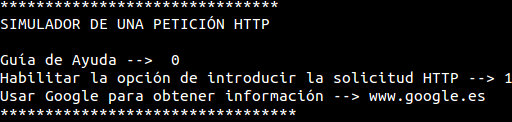
\includegraphics[width=.8\textwidth]{1}
		\caption{Inicio del programa}
	\end{figure}
	
	Como podemos observar, simplemente bastará con pulsar la tecla '0', '1' o introducir la dirección 'www.google.es' en la terminal para acceder a la opción deseada. \\
	
	
	Una vez hayamos introducido todos los campos correctamente, se mostrará el mensaje siguiente:
	
	\begin{figure}[h]
		\centering
		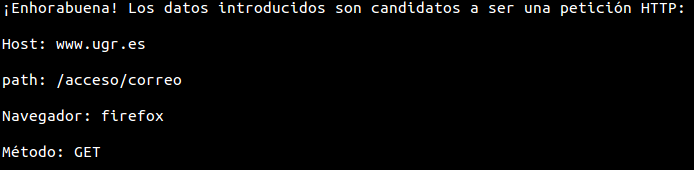
\includegraphics[width=.8\textwidth]{2}
		\caption{Petición HTTP final}
	\end{figure}
	
	Cabe destacar, que el programa no hace nada si se introduce algo que no coincida con alguna expresión regular y si introducimos una frase cuya expresión regular coincida con alguna que ya se ha introducido, se mostrará un mensaje de error.
	
	
\end{document}